\section{Forward Kinematics}
\emph{Forward kinematics} allows to compute the position and orientation of the kinematic chain given the joint parameters (e.g. angles, lengths, etc.). For instance, we can compute the position and orientation of the terminal organ given the angles of the articulations.
\begin{figure}[H]
    \centering
    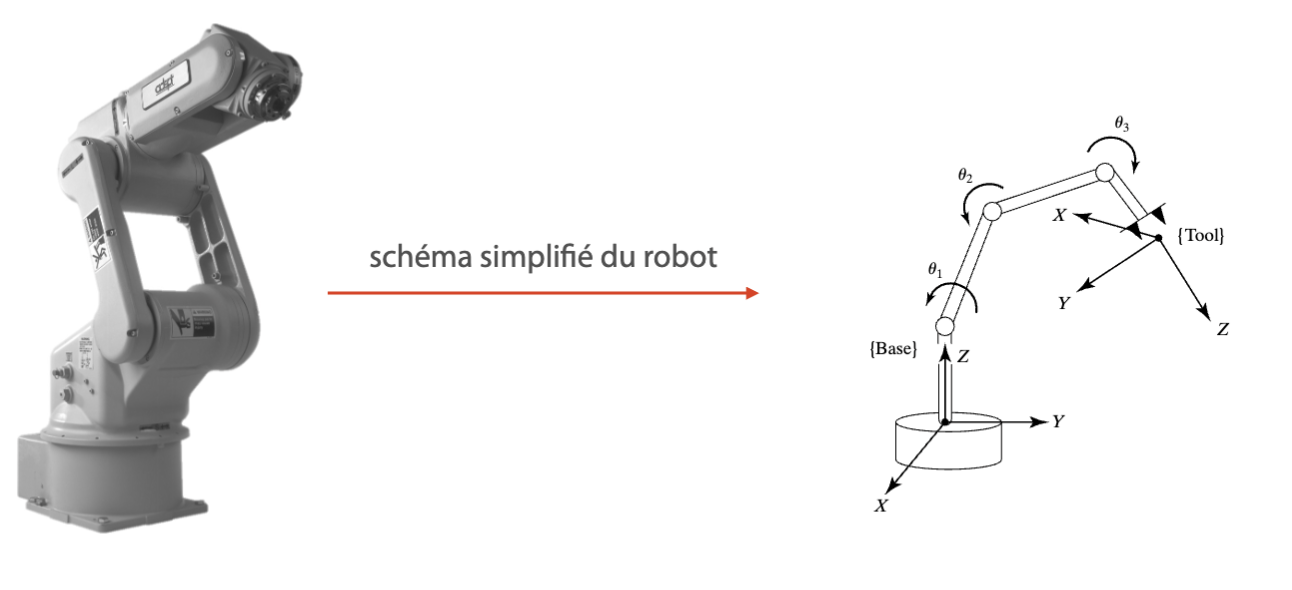
\includegraphics[width=.7\textwidth]{position/direct-kinematic.png}
\end{figure}

The kinematic chain is composed of rigid bodies interconnect by joints. The joins define the degrees of freedom of the cinematic chain, which are the parameters that we can control.
\begin{figure}[H]
    \centering
    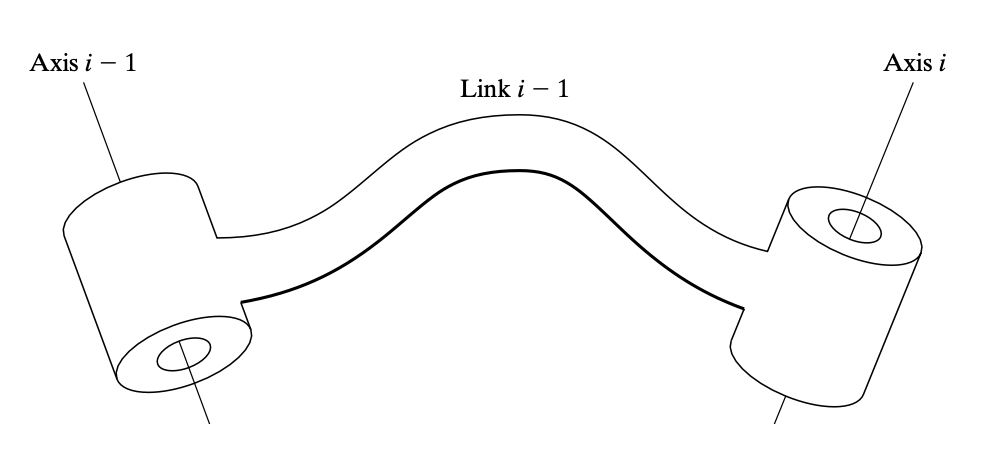
\includegraphics[width=.5\textwidth]{forward-kinematics/kinematic-chain.png}
\end{figure}